% !TeX root = tcolorbox.tex
% include file of tcolorbox.tex (manual of the LaTeX package tcolorbox)
\clearpage
\section{\tikzname\ Auxiliary Macros}\label{sec:tikzimagefilling}%
\tcbset{external/prefix=external/filling_}%
The \mylib{skins} library adds some auxiliary options to the vast option set of
\tikzname\ \cite{tantau:tikz_and_pgf}. These options can be used in any |tikzpicture|.
For the following options, the \mylib{skins} library has to be loaded
by a package option or inside the preamble by:
\begin{dispListing}
\tcbuselibrary{skins}
\end{dispListing}

See \Vref{sec:skins} for the documentation of all other options of the \mylib{skins} library.

\begin{marker}
Up to version 5.1.1 (2022/06/24) of |tcolorbox|, \tikzname\ image and picture fill extensions
were documented here. These extensions are now separate \tikzname\ libraries
and part of the \refPkg{tikzfill} package where they are documented now.
\end{marker}


\subsection{Straightening of the Arcs}

\begin{marker}
This patch is considered as an experimental feature.
It changes some of the original \tikzname\ code. This change may break
with future updates of \tikzname.
\end{marker}

\begin{docCommand}[doc new=2014-05-05]{tcbpatcharcangular}{}
The \tikzname\ package provides a nice |rounded corners| option to replace
all corners by little arcs. |\tcbpatcharcangular| is a patch which
straightens the arcs. To say it more prosaic, the little arcs are replaced
by little straight lines.

\begin{dispExample*}{sbs,lefthand ratio=0.66,right=2mm,sidebyside gap=5mm,center lower}
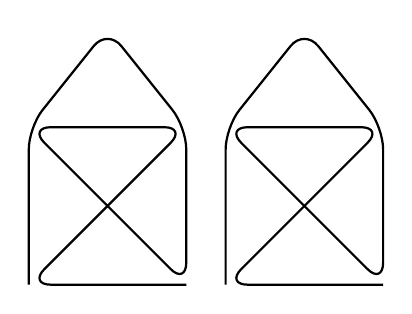
\begin{tikzpicture}
  \draw[thick,rounded corners=8pt]
    (0,0) -- (0,2) -- (1,3.25) -- (2,2) -- (2,0)
     -- (0,2) -- (2,2) -- (0,0) -- (2,0);
  \tcbpatcharcangular
  \draw[thick,rounded corners=8pt,xshift=2.5cm]
    (0,0) -- (0,2) -- (1,3.25) -- (2,2) -- (2,0)
     -- (0,2) -- (2,2) -- (0,0) -- (2,0);
\end{tikzpicture}
\end{dispExample*}

\end{docCommand}


\begin{docCommand}[doc new=2014-05-05]{tcbpatcharcround}{}
This macro reverts \refCom{tcbpatcharcangular}, i.e., the patch from
\refCom{tcbpatcharcangular} is replaced by the original code.
\end{docCommand}


\clearpage
\subsection{Extracting Node Dimensions}
The following auxiliary macros are defined by the \mylib{skins} library.
They allow to determine the width and height of an arbitrary \tikzname\ node.
To be more specific, they determine the east-to-west and the north-to-south dimensions
which may be not the maximal dimensions for a non-rectangular node.
Note that the following dimensions are measured exactly including the line width
of the border line. If a new rectangle or node with the same dimensions
and a border is to be drawn, this border width has to be subtracted.

\begin{docCommand}[doc new=2014-09-19]{tcbsettowidthofnode}{\marg{register}\marg{node}}
  Sets the east-to-west dimension of the given \meta{node}
  to the \TeX\ \meta{register}.
\end{docCommand}

\begin{docCommand}[doc new=2014-09-19]{tcbsetmacrotowidthofnode}{\marg{macro}\marg{node}}
  Defines \meta{macro} as the east-to-west dimension of the given \meta{node}.
\end{docCommand}

\begin{docCommand}[doc new=2014-09-19]{tcbsettoheightofnode}{\marg{register}\marg{node}}
  Sets the north-to-south dimension of the given \meta{node}
  to the \TeX\ \meta{register}.
\end{docCommand}

\begin{docCommand}[doc new=2014-09-19]{tcbsetmacrotoheightofnode}{\marg{macro}\marg{node}}
  Defines \meta{macro} as the north-to-south dimension of the given \meta{node}.
\end{docCommand}

\begin{dispExample}
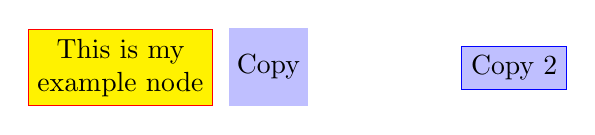
\begin{tikzpicture}
  \node[align=center,draw=red,fill=yellow] (A) {This is my\\example node};
  \tcbsetmacrotowidthofnode\mywidth{A}
  \tcbsetmacrotoheightofnode\myheight{A}
  \path[fill=blue!25!white]           %  rectangle without border
    ([xshift=2mm]A.south east)
    rectangle node{Copy} +(\mywidth,\myheight);
  \node[draw=blue,fill=blue!25!white, % standard border width 0.4pt
    minimum width=\mywidth-0.4pt,     % minus width of border
    minimum height=\myheight-0.4pt    % minus height of border
    ]
    at ([xshift=5cm]A) {Copy 2};
\end{tikzpicture}
\end{dispExample}


\subsection{Hyper Nodes}
The following auxiliary macro is defined by the \mylib{skins} library.
\enlargethispage*{1cm}

\begin{docCommand}[doc new and updated={2016-02-03}{2023-02-28}]{tcbhypernode}{\marg{macro}\marg{node}}
%  Sets the east-to-west dimension of the given \meta{node}
%  to the \TeX\ \meta{register}.
  Applies a hyperlink creating \meta{macro} from the package \refPkg{hyperref} \cite{rahtz:hyperref}
  to an existing |tikz| \meta{node}. \refCom{tcbhypernode} can only
  be used inside a |tikzpicture| environment.
  The last argument of the \meta{macro} is to be omitted and should stand
  for an object (text) which is to be made a hyperlink.
  For example, use  |\hyperref[name]| instead of |\hyperref[name]{text}|.

\begin{dispExample}
% \usepackage{hyperref}
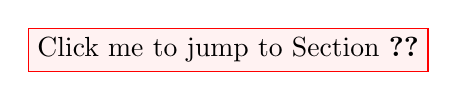
\begin{tikzpicture}
  \node[align=center,draw=red,fill=red!5] (mybutton)
    {Click me to jump to Section~\ref*{sec:tikzimagefilling}};
  \tcbhypernode{\hyperref[sec:tikzimagefilling]}{mybutton}
\end{tikzpicture}
\end{dispExample}

\end{docCommand}

